% Kilencedik és tizedik előadás

\chapter{Mobil processzorok architektúrája}

\section{Bevezetés}
A modern processzorok sok különálló egységet tartalmaznak, ezek közül a CPU-val foglalkozunk.
Mobil processzorok alatt a mobiltelefonok és a táblagépek processzorait értjük.

Csak kevés gyártó tervez mobil processzorokat és a legtöbbjük nem rendelkezik gyártási kapacitással, kivéve a Samsungot.
A többi gyártó processzorait jellemzően a TSMC vagy a Samsung gyártja le.

A mobil processzorok többsége ARM alapú, de léteznek x86 alapú mobil processzorok is.
x86 alapú processzorokkal az Intel és az AMD próbálkozott, sikertelenül (2016-ban meg is szüntették a gyártást).

\section{ARM licenszek}
Az ARM processzorok gyártóinak két lehetősége van:
\begin{itemize}
    \item Cortex licensz felhasználása
    \item Architektúra licensz felhasználása
\end{itemize}

Cortex licensz esetén a vásárló egy komplett mikroarchitektúra tervet kap meg, konfigurálható opciókkal.
Az architektúra licensz viszont csak arra jogosítja fel a vásárlót, hogy az utasításkészletet használja.

\section{Az ARM alapú mobil processzorok fejlődése}
Az ARM ISA fejlődésével együtt az ARM mobil processzorok is fejlődtek.
Ennek az egyik fontos állomása volt a v7-ről v8-ra átállás, ami behozta a 64 bites támogatást.
Az áttérés során a cégek előtt két út állt:
\begin{itemize}
    \item egyesek megtartották a hagyományos szimmetrikus többmagos felépítést
    \item mások egyúttal áttértek a big.LITTLE architektúrára is
\end{itemize}
Az Apple és a MediaTek szimmetrikus megvalósítást alkalmazott, a Samsung és a Huawei pedig big.LITTLE architektúrát kezdett használni.
A 64 bites áttérés tehát nagyjából egyszerre történt a big.LITTLE átállással, 2013 és 2016 között.

Nem sokkal ezután történt az átállás az ARMv8.2-re (2018), ami a dinamikus magklaszterek használatával jelentős teljesítmény növekedést ereményezett.
Ezzel egyidőben jelentek meg az ARM szerverprocesszorok is.

\section{Az Intel Atom és az AMD Cat család}
Az Intel és AMD hagyományos processzorai a nagy fogyasztás miatt nem voltak alkalmasak a mobil felhasználásra, ezért az Intel 2008-ban, az AMD pedig 2011-ben új processzorokkal állt elő.
Az AMD piacra lépése nagyon későinek számított.

Az Intel Atom processzora a hagyományos processzorokkal ellentétben 2 és 3 széles volt, ennek oka az alacsonyabb fogyasztás.

Ezek ellenére egyik cég se tudott érdemben betörni a mobil piacra, ezért 2015-ben befejezték ezeket a fejlesztéseket.

\section{Windows táblagépekre fejlesztett Core 2 processzorok}
2013-tól a Microsoft megjelent a Surface táblagépekekkel, amik 2 az 1-ben gépek voltak.
Intel processzorokkal szerelték őket, először 2, aztán 4 maggal.
A táblagépek között nagyjából 10\%-os részesedést értek el.

Az elmúlt néhány évben a Windows tabletek is megjelentek Qualcomm ARM processzorokkal.
A céljuk olyan 2 az 1-ben gépek megalkotása, amik nagyon hosszú üzemidővel rendelkeznek (Always on, always connected).
Fő problémájuk a szoftver kompatibilitás.

\section{ARM processzorok az Apple Mac eszközeiben}
Az Apple 2006-tól az Inteltől vásárolta a processzorait.
2020-ban viszont bejelentették, hogy saját processzort fog fejleszteni a MacOS alá.
Az új processzor, az Apple M1 jó teljesítménnyel rendelkezik.

\section{Mobil processzor architektúrák fejlődése}
A fejlődésnél négy fő szakaszt különböztetünk meg:
\begin{itemize}
    \item egymagos processzorok
    \item szimmetrikus többmagos processzorok
    \item big.LITTLE processzorok
    \item DynamIQ klaszter alapú processzorok
\end{itemize}

Az egymagos processzorok használata kb. 2003-tól 2010-ig tartott, általában 32 bitesek voltak.
A többmagos processzoroknál először szimmetrikus felépítést alkalmaztak, 2011-2013-ban, amik szintén 32 bitesek voltak.
A big.LITTLE architektúra 2013-2016-ig tartott, itt megtörtén a 64 bites átállás.
DynamIQ processzorokat 2018-tól gyártanak.

Az egymagos processzorokat nem tárgyaljuk.

\subsection{Szimmetrikus többmagos processzorok}
A desktop processzorok többmagossá válása után kb. 6 évvel, 2011-ben jelentek meg a mobiloknál is a többmagos felépítések.
Cél a teljesítmény növelése.
Az egyik első ilyen rendszer a Samsung Exynos 4412 volt.
\begin{figure}[H]
    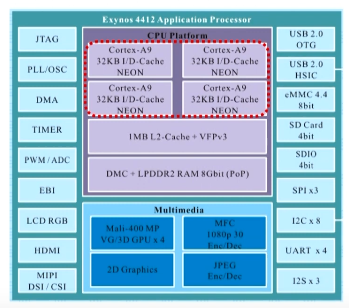
\includegraphics[width=0.8\textwidth]{exynos}
    \centering
    \caption{A Samsung Exynos 4412 felépítése}
    \label{fig:exynos}
\end{figure}
A szimmetrikus többmagos processzorok fő fejlesztési iránya a magok számának növelése volt, a kezdeti 2-ről 4-re, majd 8-ra emelkedett.

Az általános felépítés kettő vagy négy magos magklasztereket jelentett, a klaszteren belül egy közös L2 cache-el.
8 magos rendszereket 2x4 magos klaszterrel készítettek.

\subsection{big.LITTLE architektúrák}
A kifejesztésük fő motivációja a fogyasztás csökkentése.
Az ötlet onnan eredt, hogy az okostelefon használata során nagyon gyakran változik a teljesítmény igény.
Ezért kétféle magot hoztak létre, kis fogyasztású, kis teljesítményűt és nagyobb fogyasztású de nagyobb teljesítményűt.

\subsubsection{Feladatok elosztása}
Az így létrejövő heterogén többmagos rendszerekben a feladatokat többféle módon is fel lehet osztani a magok között:
\begin{itemize}
    \item mester-szolga elv
    \item feladattovábbítás a dedikált végrehajtók felé
    \item más típusú processzor felhasználása
\end{itemize} 

A mester-szolga elvnél van egy megkülönböztetett mester mag és egy vagy több szolga mag.
Ekkor a mester mag látja el a feladatok kiosztását is.
Az IBM, Sony és a Toshiba próbálkozott ilyen elvű processzorral (Cell processzor), de a bonyolult programozás miatt nem volt túl működőképes.

A második esetben a processzorban dedikált végrehajtóegységek vannak, mint pl. GPU.
Minden utasítás ahhoz az egységhez kerül, ami a legalkalmasabb a végrehajtására.

Az utolsó működést tipikusan big.LITTLE architektúráknál használják, ekkor különböző típusú CPU-k működnek együtt.

\subsubsection{big.LITTLE alapelvek}
A big.LITTLE processzorokban kettő vagy több magklaszter dolgozik, amik architekturálisan megegyező magokat tartalmaznak.
A magklaszterek cache koherens módon vannak összekötve.
Ehhez kell egy szoftver, ami a klasztereket vezérli.

\subsubsection{Működési elv}
A big.LITTLE technológia különböző módokon implementálható, mi az exkluzív klaszter kapcsolást vizsgáljuk a működési elv leírásánál.
Feltételezzük még, hogy egy klaszter minden magja azonos munkaponton dolgozik.
\begin{itemize}
    \item egy kernel rutin figyeli a teljesítmény igényt és kiválasztja a megfelelő munkapontot
    \item ha a teljesítmény igény kicsi, a kis klaszter van használatban
    \item ha a teljesítmény igény megnő, klaszter átkapcsolás történik a nagy magokra
    \item ha újra elég a kisebb teljesítmény, a klaszter visszavált a kis magokra
\end{itemize}
Egyszerre csak egy klaszter működhet, ezért ez az exkluzív klaszter kapcsolási rendszer.

\subsubsection{Megvalósítás}
A technológia hardverkövetleményei:
\begin{itemize}
    \item a kis és nagy klasztereknek architektúrálisan azonosnak kell lennie
    \item a gyors átkapcsoláshoz szükséges egy cache koherens megoldás
    \item a megengedett magszám klaszterenként általában 4
    \item megfelelő szoftvertámogatás szükséges, amit a processzorgyártó ad át a gyártóknak, kernel kiegészítések formájában
\end{itemize}

A big.LITTLE architektúrákat három szempont szerint viszgáljuk:
\begin{itemize}
    \item klaszterek és magok száma
    \item ütemezési megoldások
    \item feszültség és frekvencia ellátás
\end{itemize}

Mag klaszterek szerint két vagy három klaszteres rendszereket különböztetünk meg.
Az egyes klaszterekben 1, 2, 3 vagy 4 mag lehet.

Az ütemezési megoldások vizsgálatánál egy 2 klaszteres processzort tekintünk.
Az ütemező működhet klaszter vagy mag alapon.
Mindkét esetben kétfajta implemtáció lehet: exkluzív és inkluzív.
Exkluzívnál vagy egyik, vagy másik klaszter van hozzárendelve egy adott feladathoz.
Inkluzívnál megengedett, hogy a két klaszter egyszerre működjön nagy teljesítmény igény esetén.
Általában exkluzív implementációt használnak, mivel az inkluzívat nehezebb implementálni és viszonylag kis gyorsulást eredményez.

A mag alapú ütemezés is történhet exkluzív vagy inkluzív módon.
Exkluzív mag allokációnál a magokat kis-nagy párokba szervezik.
Az ütemező a terheléstől függően a nagy vagy kis magot választja ki.
Inkluzívnál viszont minden mag külön-külön aktiválható, ezért ez egy globális ütemező.
Ma ez a legelterjedtebb.

A felhasználói igény döntően a frekvenciát dönti el, ami meghatározza a szükséges feszültséget.
A szabályzás üzemeltethet minden magot azonos feszültségen és frekvencián, szabályozhatja magonként a frekvenciát, közös feszültséget tartva, vagy magonként különböző frekvencia és feszültség beállításokat alkalmazhat.
A leghatékonyabb az utolsó megoldás.

\subsection{DynamIQ magklaszterek}
Az ARM 2013-ban kezdte el fejleszteni a technológiát, 2018-ban kezdték használni.
Ez jelenti a big.LITTLE architektúrák utáni lépcsőfokát a fejlődésnek.

A dinamikus magklaszter két különböző magot képes tartalmazni: kis mag és nagy mag.
Különbség a big.LITTLE klaszterekhez képest, hogy a magokat közel tetszőlegesen lehet párosítani.

\subsubsection{Energy Aware Scheduling}
A fogyasztást egy intelligens fogyasztáscsökkentő eljárás bevezetésével javította, ez az EAS - Energy Aware Scheduling.
Ez előtt a Linux kernel a CFS-t, azaz a Completely Fair Schedulert használta, ami elsőrorban teljesítményre optimalizált.
Hátránya, hogy heterogén rendszerekben nem működik elég hatékonyan.
Az EAS ezzel szemben figyelembe veszi a big.LITTLE felépítést, így elérve a lehető legalacsonyabb fogyasztást.

\subsubsection{DynamIQ klaszterek jellemzői}
\begin{itemize}
    \item ARMv8.2-t támogatnak
    \item két típusú magot tartalmazhatnak a klaszterek
    \item magonkénti L2 cache-el rendelkezik - ez lényegesen jobb megoldás, mint a közös L2 cache
    \item megjelenik a harmadik szintű gyorsítótár, a magok közös L3 cache-el rendelkeznek
    \item a klaszter egy új egységet is tartalmaz, ez a DSU (Dynamic Shared Unit): ebben van az L3 cache és egy snoop filter, ami a cache koherencia fenntartását teszi hatékonyabbá. Következmény, hogy alacsonyabb késleltetéssel érhetők el a gyorsítótárak.
    \item a magok partícionálhatók: négy partíció hozható létre, amik magokat, külső gyorsítókat és az L3 cache bizonyos részeit tartalmazzák. A partíciókat feladatok szerint lehet kialakítani.
    \item finomabb feszültség-frekvencia szabályozás, a különböző partíciók eltérő frekvencián és feszültségen működhetnek
\end{itemize}

\section{Magok szélességének fejlődése}
A processzormagok két részre bonthatók: frontend és backend.
A frontend több utasítást dolgoz fel szekvenciálisan és küldi ki a backend számára.
A backendben egyedi utasítások kerülnek feldolgozásra a megfelelő futószalagokon.
A mag szélessége a mag legszűkebb keresztmetszetét jelöli, ami legtöbbször a dekódoló szélességének felel meg.
Teljesítmény szempontjából minél szélesebb egy mag, annál gyorsabb a processzor, a fogyasztás viszont fordítva működik.
Fontos szempont még, hogy a mag tud-e többszálas működést.
A szálak gyorsító hatása az adott felhasználástól függ.

Az első mobil rendszerekben (2000-es évek eleje) 2-3 széles processzorok dolgoztak.
Ez nem sokat változott a 64 bites átállással, mivel a kisebb teljesítményű rendszerek maradtak 2 szélesek, a nagyobb teljesítményűek pedig 3 szélesek.
Ezután az Intel és az AMD megjelentek a saját mobil processzoraikkal, amik 2 szélesek voltak, viszont nem voltak versenyképesek.

Az ARMv8 és v8.2 ISA-ra épülő processzoroknál a magasabb teljesítmény érdekében áttértek 4-es és 5-ös szélességre.
Ennek eredménye, hogy a kibocsátási és a kiküldési ráta is jelentősen megnőtt.
A szélesség növeléséhez növelni kellett az erőforrásokat, így a ROB méretét is.
Ezzel együtt megjelent a MOP cache, ami a már dekódolt utasításokat tudja tárolni és újrahasználni, pl. elágazásbecslés visszatörlésnél vagy ciklusnál.

Az Apple nagyon hamar, az A7 processzorukban (2013) áttért a 6 széles magokra.
Ezzel teljesítményben minden más processzort leelőzött, amit később tartott is.
Később az A11 és A12X processzorokban 7-es, majd az A13, A14 és M1 processzorokban 8-as szélességű magokat alkalmaztak.

A Samsung szintén nagy lépésekkel fejlődött a Mongoose processzorával, 6-os szélességet értek el, a 8 széles processzoruk fejlesztését viszont leállították.

Az AMD hagyományos desktop architektúrái ezzel szemben csak 4 szélességig fejlődtek (Bulldozer család), az Intelek viszont 6-ig (Alder Lake).
Az AMD ezzel sokat veszített a piacból.
Tehát a mobil processzorok szélesebbek a hagyományos rendszerknél.
Ennek oka, hogy a hagyományos rendszerek CISC architektúrák, ahol változó hosszúak az utasítások.
A RISC-ek ezzel szemben fix utasításhosszal rendelkeznek, ezeket pedig sokkal könnyebb dekódolni.

\subsection{A Samsung Mongoose családjának fejlődése}
A Samsung 2010-ben alapított egy processzor fejlesztő központot Austinban, ahol a Mongoose családot fejlesztették.
Első megjelent processzoruk volt az ARMv8 alapú M1, 2016-ban.
Később áttértek az ARMv8.2-re, majd az M6-al leálltak a fejlesztéssel.
Az elkészült processzorokat a Samsung Galaxy telefonokban használták.
A több száz alkalmazott mérnök ellenére a Samsung 2019-ben bezárta a központot, utána pedig publikálták a processzorok fejlődését.

Az első Mongoose processzor a Galaxy S7-ben jelent meg, az utolsó pedig a Galaxy S20-ban (2020).
Kiemelt ezek közül az M3-as mag, amivel a Samsung áttért az ARMv8-ra.
A 10 éves fejlesztés során a teljesítmény növelését három területen keresték:
\begin{itemize}
    \item kisebb igényű feladatok végrehajtásának gyorsítása: ezen a területen arra jutottak, hogy az előlehívás és a cache koherencia protokollok optimalizálásával lehet gyorsulást elérni
    \item közepes igényű feladatok: itt az elágazás kezelés és a cache fejlesztésével tudtak eredményeket elérni
    \item nagy igényű feladatok: ezeknél főleg a szélesség növelésével és a megfelelő erőforrások biztosításával lehetett gyorsítani
\end{itemize}
Ezeknek a szempontoknak a figyelembevételével az M6 az M1-hez képest 2,71-szer nagyobb IPC-t (Instruction per Cycle) ért el.
Ez évente 20\%-os növekedésnek felel meg.

A teljesítményt a programfutások trace-elésével vizsgálták és ezek alapján állapították meg a fejlesztési lehetőségeket.

\subsubsection{A mikrooperációs cache}
A magok szélességének növelésével szükségessé vált az utasítások gyorsítótárazása, ezért az M5 bevezetta a mikrooperációs cache-t.
Ez 384 utasítást tudott tárolni, a használatával a cache-elt utasításoknál megspórolható a lehívás és a dekódolás.
A többi gyártóhoz képest későn vezették be.

\subsubsection{Végrehajtó egységek száma}
A szélesség duplájára növelésével a végrehajtó egységek is lépést tartottak, itt is kb. kétszeres növekedés ment végbe.

\subsubsection{Összegzés}
A fejlesztések ellenére az ARM processzorok gyorsabban fejlődtek, ezért a Samsung is visszatért ezek használatára és felhagyott a saját fejlesztéseivel.

